%% The first command in your LaTeX source must be the \documentclass command.
%%
\documentclass[jec]{acnsart}

% 允许更灵活的断行以避免 overfull hbox
\tolerance=1000
\emergencystretch=3em
\hfuzz=2pt
\sloppy

% 抑制部分无害警告
\usepackage{silence}
\usepackage{amsmath}
\usepackage{amssymb}
\usepackage{graphicx}
\usepackage{placeins}

% 让LaTeX更积极地放置浮动体
\renewcommand{\topfraction}{0.95}
\renewcommand{\bottomfraction}{0.95}
\renewcommand{\textfraction}{0.05}
\renewcommand{\floatpagefraction}{0.8}

% 减少图表与正文之间的间距
\setlength{\textfloatsep}{4pt plus 1pt minus 1pt}
\setlength{\floatsep}{4pt plus 1pt minus 1pt}
\setlength{\intextsep}{4pt plus 1pt minus 1pt}
\setlength{\abovecaptionskip}{3pt}
\setlength{\belowcaptionskip}{1pt}

\graphicspath{{./figures/}{figures/}{./}}
\WarningFilter{hyperref}{Ignoring empty anchor}
\WarningFilter{scrartcl}{Incompatible usage}
\WarningFilter{pdfx}{Setting all color commands}
\WarningFilter{doclicense}{The pdfx package was detected}
\WarningFilter{mathdesign}{No font specified}
\WarningFilter{mathdesign}{`bookman' option not defined}

\setdoi{10.55056/jec.ARTNUM}
\setjournalyear{2025}
\setjournalvolume{1}
\setjournalissue{1}
\setcounter{page}{1}


%%
%% end of the preamble, the start of the body of the document source.

%%
%% The "title" command
\title{Physics-Guided Contrastive Learning for Wearable Fall Detection: Toward Low-Latency On-Device Inference}

%%
%% The "author" command and its associated commands are used to define
%% the authors and their affiliations.

% Authors and affiliations removed for anonymous review
\author[1]{Anonymous Author(s)}
\address[1]{Anonymous Institution}

\begin{document}

%%
%% The abstract is a summary of the work to be presented in the
%% article.
\begin{abstract}
Wearable edge devices for fall detection must balance high sensitivity with stringent latency, memory, and energy constraints. PhyCL-Net uses a time-domain architecture employing a Physics-Guided Dynamic Kernel (PDK) and Jerk-aware Fall-Aware Attention (FAA), removing the explicit spectral feature branch. Training uses hierarchical dual-view contrastive regularization, with only the core model retained during deployment. On SisFall with 12-fold LOSO validation, PhyCL-Net achieves 98.21\%$\pm$0.10\% accuracy and 98.16\%$\pm$0.10\% Macro-F1 across five seeds, requiring 1.049M parameters and 0.15 GFLOPs, with median CPU latency reduced by 31.6\% to 125.99\,ms compared to the spectral baseline. Constraint-based ROC analysis gives FPR of 0.72\% at 95\% TPR and a 2.73-percentage-point reduction in TPR at FPR${=}$1\% relative to the spectral baseline. These ROC summaries characterize empirical discrimination under common reference constraints. Supplementary prototype summaries report p95 processing latencies of 78.6\,ms on Pi Zero 2 W and 94.7\,ms on Apollo4, supporting further development toward low-latency on-device inference. These timings describe the reported processing paths; integrated sensing-to-alert latency remains a separate evaluation target.
\end{abstract}

%%
%% Keywords. The author(s) should pick words that accurately describe
%% the work being presented. Separate the keywords with commas.
\begin{keywords}
  Edge AI \sep
  Wearable Fall Detection \sep
  Physics-Inspired Deep Learning \sep
  Contrastive Learning \sep
  Real-Time Inference \sep
  Resource-Constrained Deployment
\end{keywords}

%%
%% This command processes the author affiliation and title
%% information and builds the first part of the formatted document.
\maketitle

\section{Introduction}

Falls represent a leading cause of injury-related morbidity among older adults, with significant healthcare costs and quality-of-life implications~\cite{Bergen2016Falls}. Wearable sensor-based fall detection has emerged as a promising approach for continuous monitoring~\cite{Wu2015Wearable}, and comprehensive surveys have reviewed the development of detection methodologies~\cite{Ramachandran2020Survey,mubashir2013survey}. However, deploying such systems on resource-constrained edge devices introduces fundamental trade-offs between detection accuracy and computational efficiency.

Deep learning has been widely studied for sensor-based activity recognition~\cite{wang2019deep}. ResNet introduced residual learning for image recognition~\cite{he2016resnet}, while LSTM introduced a recurrent architecture for learning long-term dependencies~\cite{hochreiter1997lstm}. Transformers were introduced for sequence transduction~\cite{Vaswani2017Attention}; their advantages over simpler architectures have been questioned specifically in long-term time-series forecasting~\cite{Zeng2023TransformersEffective}, a different task from fall classification. Fall-detection studies include a CNN--GRU ensemble~\cite{Liu2023FallEnsemble} and a comparison of LSTM with CNN-based transfer learning~\cite{Butt2022FallLSTM}.

Time- and frequency-domain representations have been combined in contrastive time-series pre-training~\cite{Zhang2022TFC}. An explicit spectral branch adds computation whose runtime cost depends on the implementation and platform. The challenge is compounded by alarm fatigue in clinical settings~\cite{Cvach2012AlarmFatigue}, where excessive alarms can burden staff and reduce responsiveness; this clinical evidence motivates attention to false alarms without directly quantifying wearable alarm burden. As shown later in the experimental results, removing the explicit spectral feature branch reduces median CPU latency by 31.6\% but decreases constraint-based ROC TPR at FPR${=}$1\% by 2.73 percentage points, illustrating the accuracy--efficiency trade-off.

Wearable fall-detection methods exploit changes in acceleration and body orientation~\cite{Wu2015Wearable}. This motivates temporal-difference features as candidate transient cues, without assuming that jerk alone reliably distinguishes falls from vigorous activities of daily living. Architectural innovations including channel attention~\cite{hu2018squeeze}, spatial-channel attention~\cite{woo2018cbam}, and adaptive kernel selection~\cite{li2019sknet} provide architectural precedents for feature recalibration; applying them to temporal fall signals is a design adaptation from the original visual-recognition setting.

SimCLR established an augmentation-based contrastive framework for visual representations~\cite{chen2020simclr}. Time-series formulations include temporal and contextual contrasting~\cite{Eldele2021TSTCC} and time-frequency consistency~\cite{Zhang2022TFC}. The effectiveness of time-series augmentation depends on the method and dataset~\cite{Iwana2021DataAugmentation}. Transfer learning and domain adaptation have improved activity recognition or time-series classification under the settings evaluated in those studies~\cite{Jia2024TransferLearningHAR,Wu2024DomainAdaptationContrastive}; these findings do not guarantee robustness to arbitrary sensor configurations.

Building on these foundations, we propose PhyCL-Net, a physics-inspired time-domain network designed for studying the accuracy--cost trade-off in wearable fall detection. The architecture centers on two lightweight components:
\begin{enumerate}
\item Physics-Guided Dynamic Kernel (PDK) adapts temporal receptive fields according to local signal dynamics, enabling efficient multi-scale feature extraction.
\item Jerk-aware Fall-Aware Attention (FAA) combines temporal-difference cues and axis attention to emphasize candidate transient segments.
\end{enumerate}

A training-only hierarchical dual-view contrastive objective is used to encourage class separability, with auxiliary heads removed during inference to avoid additional deployment cost.

PhyCL-Net achieves 98.21\%$\pm$0.10\% accuracy and 98.16\%$\pm$0.10\% Macro-F1 on SisFall with 12-fold LOSO validation. The model contains 1.049M parameters, requires 0.15 GFLOPs, and achieves 125.99\,ms p50 latency (31.6\% reduction vs.\ spectral baseline). Under the common ROC reference constraints, FPR is 0.72\% at TPR${=}$95\%; TPR at FPR${=}$1\% is 2.73 percentage points lower than the spectral baseline.

The principal contributions are:
\begin{itemize}
\item Low-latency on-device inference as an engineering objective, with parameters, FLOPs, and CPU latency reported alongside accuracy and supplementary prototype processing times.
\item Physics-inspired modeling through PDK and FAA, which utilize physical priors for class discrimination without an explicit spectral feature branch.
\item Training-only contrastive regularization, with auxiliary heads removed after training to preserve zero deployment overhead.
\item Constraint-based operating-point analysis, using common sensitivity and false-positive-rate targets to characterize empirical score trade-offs relevant to continuous monitoring.
\end{itemize}

\section{Related Work}

Wearable fall-detection research includes threshold methods and feature-based classifiers~\cite{mubashir2013survey}, with deep learning studied extensively in sensor-based activity recognition~\cite{wang2019deep}. Examples of deep fall-detection methods include a CNN--GRU ensemble~\cite{Liu2023FallEnsemble} and LSTM and CNN-transfer approaches~\cite{Butt2022FallLSTM}. Accuracy alone does not determine wearable suitability; latency, memory, energy, and the deployed decision rule also require evaluation.

Another important line of work improves discriminability through spectral or time--frequency preprocessing. These representations can highlight transient structure, and they are often paired with increasingly expressive sequence models. However, from an edge-deployment perspective, preprocessing is not free: extra transforms increase memory traffic, implementation burden, and runtime variability. For this reason, our comparison is not between ``deep learning'' and ``classical'' methods in the abstract, but between a matched spectral baseline and a lighter time-domain alternative under a common protocol.

Recent research has evaluated augmentation, contrastive learning, and transfer-oriented objectives for time-series learning under the respective experimental settings~\cite{Eldele2021TSTCC,Iwana2021DataAugmentation,Jia2024TransferLearningHAR,Wu2024DomainAdaptationContrastive}. In the present study, the contrastive component is used only during training, and the cross-dataset results are reported as supplementary transfer evidence that complements the primary LOSO study and helps characterize behavior beyond the main benchmark setting. This framing keeps the contribution aligned with the evidence presented in the manuscript.

\section{Methodology}

This section isolates the proposed architecture and its training objective. The problem is formulated as a window-based time-series classification task. Each sample $(X_i, y_i)$ consists of an inertial window $X_i \in \mathbb{R}^{C \times T}$ and binary label $y_i \in \{0,1\}$. Training minimizes class-weighted cross-entropy loss together with the training-only contrastive regularizer introduced later in this section.

\FloatBarrier
\subsection{Overview of PhyCL-Net}
PhyCL-Net is a compact time-domain backbone comprising a lightweight stem and three stages that progressively downsample the time domain. For input $X \in \mathbb{R}^{B \times 3 \times 512}$, the stem applies GhostConv1d ($k{=}5, s{=}1, p{=}2$), mapping 3 to 48 channels while preserving $T{=}512$. Stage~1 operates at $(C,T){=}(48, 512)$ with two PhyCL-Blocks. Transition layers use SeparableConv1d ($k{=}5, s{=}2, p{=}2$) for downsampling. Stage~2 operates at $(96,256)$ and Stage~3 at $(192,128)$, each with two PhyCL-Blocks. The head uses AdaptiveAvgPool1d(1), Linear (192 to 2), and Softmax for classification.

Each PhyCL-Block comprises two processing streams: the Physics-Guided Dynamic Kernel (PDK), which adapts temporal receptive fields to local signal dynamics, and the Jerk-Aware Fall-Aware Attention (FAA), which emphasizes high-jerk intervals. The outputs are integrated using symmetric cross-gated fusion with a residual connection and learnable scaling. Figure~\ref{fig:architecture} illustrates the overall architecture of PhyCL-Net, showing how the input signal flows through the PDK and FAA branches before being fused via the Cross-Gated Fusion Unit. The figure also provides a detailed view of the internal structure of a single PhyCL-Block, highlighting the two parallel processing streams---the Physics-Guided Dynamic Kernel (PDK) for multi-scale temporal adaptation and the Jerk-aware Fall-Aware Attention (FAA) for transient emphasis---and their integration through the symmetric cross-gated fusion unit.

\begin{figure}[!htbp]
\centering

\includegraphics[width=0.85\linewidth]{figures/fig01_architecture_and_block.pdf}
\caption{The overall architecture of PhyCL-Net. Within each PhyCL-Block, the feature input is processed by two parallel branches: the Physics-Guided Dynamic Kernel (PDK) for adaptive receptive fields and the Fall-Aware Attention (FAA) for smoothed temporal-difference cues and axis attention, fused via the Cross-Gated Fusion Unit. The detailed internal structure of a single PhyCL-Block is also shown, illustrating the two parallel streams (PDK for multi-scale temporal adaptation and FAA for transient emphasis) and their integration through the symmetric cross-gated fusion unit. The proposed model has no active MSPA frequency-feature branch; the dashed path carries 10 temporal and two rFFT routing descriptors. FAA retains Gaussian smoothing ($k=5$), first and second differences, and axis attention; fusion uses three global gate MLPs and a $k=7$ spatial gate before the scaled residual addition.}
\label{fig:architecture}
\end{figure}

\FloatBarrier

\subsection{Physics-Guided Dynamic Kernel (PDK)}
Acceleration and orientation changes motivate analysis at more than one temporal scale~\cite{Wu2015Wearable}. A single fixed kernel can restrict the temporal contexts represented under a limited compute budget. PDK addresses this by routing features through a small set of depthwise 1D temporal kernels (convolutions focused on individual input channels over time) with sizes $\{7, 15, 31, 63\}$, inspired by selective kernel networks~\cite{li2019sknet}. This near-doubling progression was chosen as a compact multi-scale set that spans short impact-like transients through longer post-impact evolution while keeping the branch count small enough for edge inference. It then combines their outputs with input-dependent mixture weights (values that determine each kernel's influence).

The mixture weights are predicted from two lightweight signals: (i) a compact 12-dimensional descriptor $p=\phi(F)\in\mathbb{R}^{12}$, extracted from the block input $F$, comprising 10 temporal descriptors and two rFFT-derived descriptors (spectral centroid and high-frequency energy ratio), and (ii) a 4-way complexity logit $\ell^{\mathrm{cmp}}$ predicted from global average pooled features. A three-layer physics MLP ($12{\rightarrow}32{\rightarrow}32{\rightarrow}4$) maps $p$ through a final sigmoid gate to $w^{\mathrm{phy}}\in\mathbb{R}^{4}$, while a two-layer complexity MLP ($C{\rightarrow}32{\rightarrow}4$) produces $\ell^{\mathrm{cmp}}$. Their element-wise product is normalized via a learnable softmax temperature $\tau_{\mathrm{dks}}=\max(0.1,\tilde{\tau}_{\mathrm{dks}})$ (initialized to 1.0) to obtain the final routing weights $a=\mathrm{Softmax}((\ell^{\mathrm{cmp}}\odot w^{\mathrm{phy}})/\tau_{\mathrm{dks}})$. The PDK output is then computed as:
\begin{equation}
\label{eq:pdk}
\mathrm{PDK}(F) = \sum_{k\in\mathcal{K}} a_k\, \mathrm{DWConv}_{k}(F), \quad \mathcal{K}=\{7,15,31,63\},
\end{equation}
where $\mathrm{DWConv}_{k}$ denotes the depthwise temporal-kernel branch with kernel size $k$, $\mathrm{GAP}(\cdot)$ is AdaptiveAvgPool1d(1), and $\odot$ denotes element-wise multiplication. Equation~\ref{eq:pdk} describes the adaptive kernel mixture, with branch normalization and subsequent feature refinement omitted from this schematic notation. The feature convolutions operate in the time domain. The routing descriptor retains two rFFT-derived quantities, spectral centroid and high-frequency energy ratio; these control the kernel weights and do not form a separate frequency-feature branch. Figure~\ref{fig:pdk_module} depicts the detailed structure of the PDK module, illustrating how features are routed through multiple temporal kernels with input-dependent mixture weights derived from physics descriptors.

\begin{figure}[!htbp]
\centering
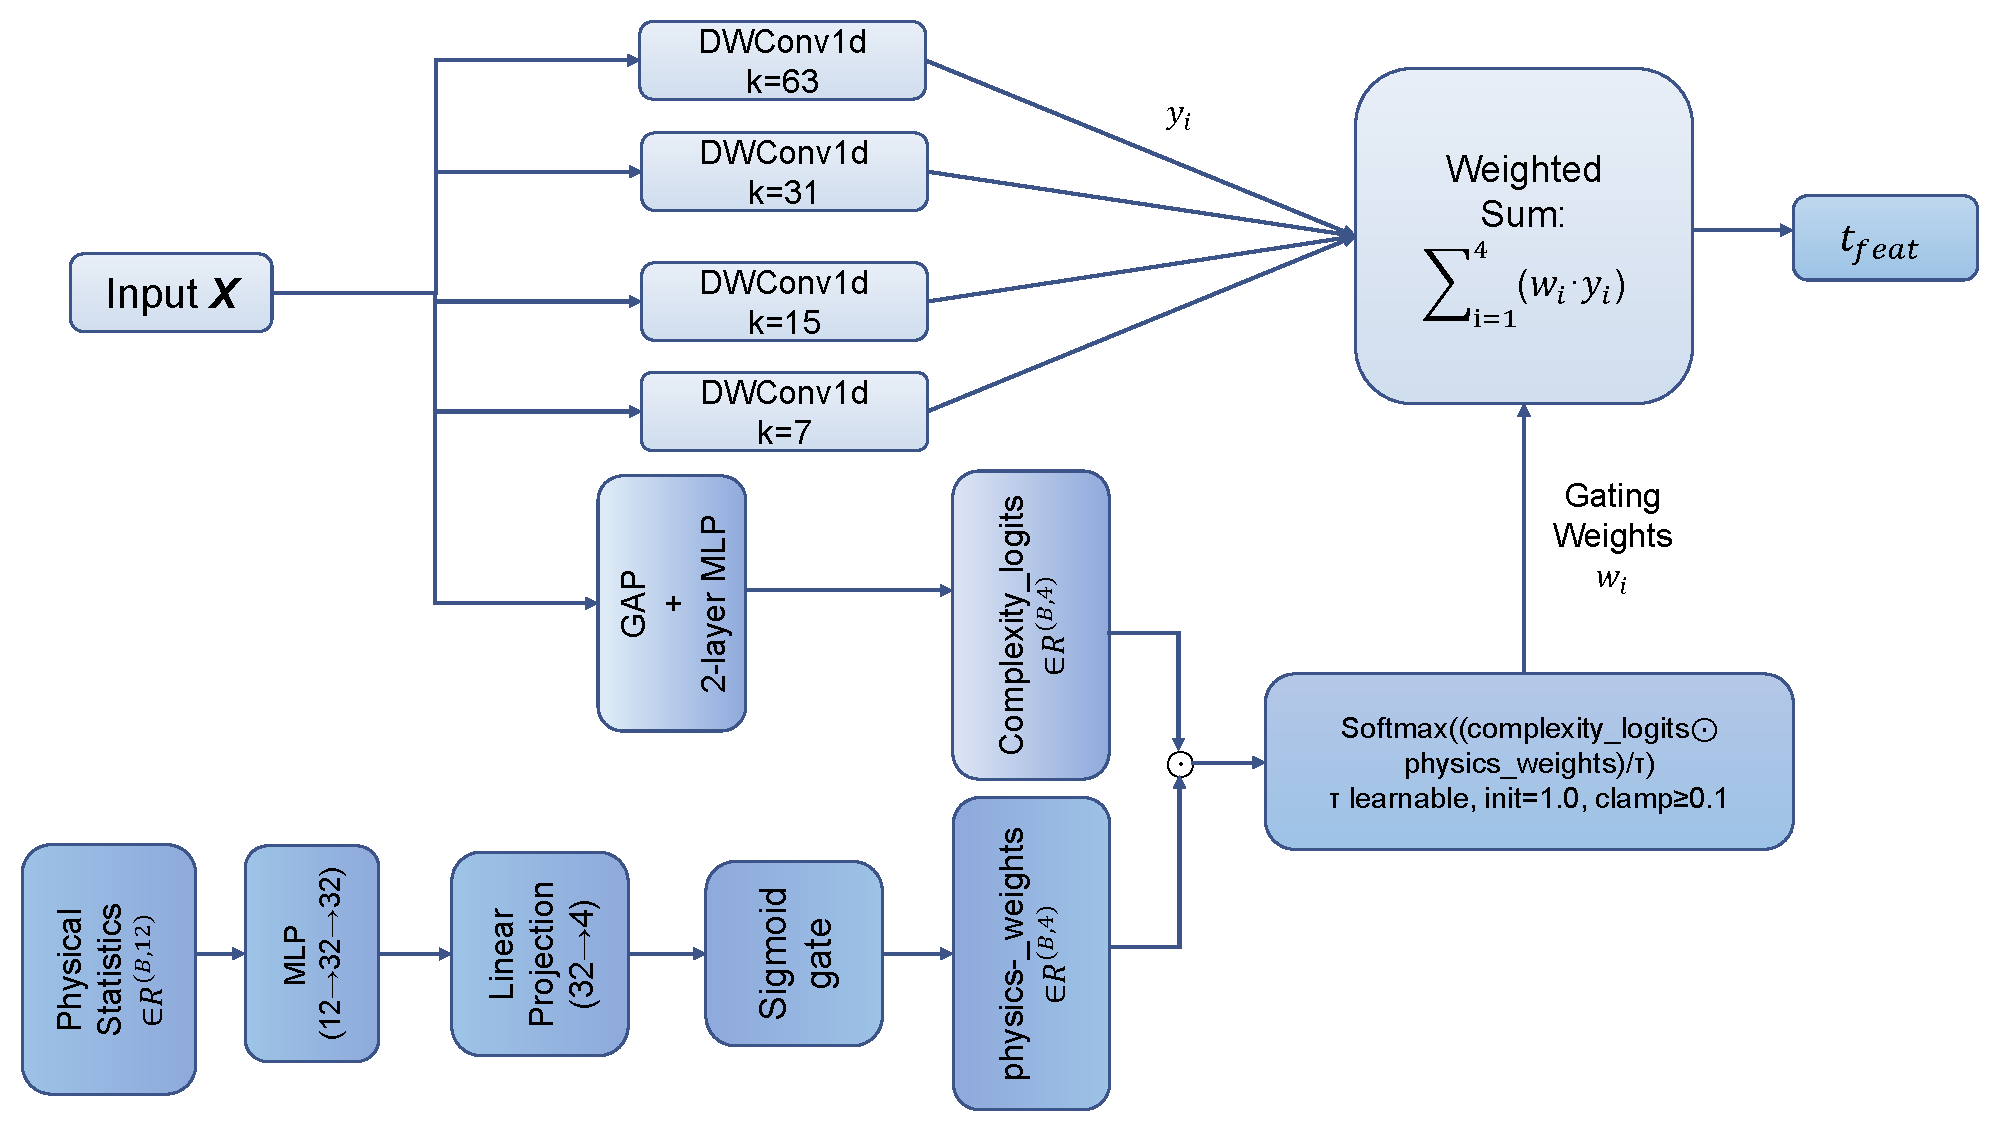
\includegraphics[width=0.85\linewidth]{figures/fig02_pdk_module.pdf}
\caption{Physics-Guided Dynamic Kernel (PDK) module with Dynamic Kernel Selection (DKS). The module routes features through multiple temporal kernels with input-dependent mixture weights derived from physics descriptors. The diagram's input $X$ denotes the block feature input $F$ in Eq.~\ref{eq:pdk}.}
\label{fig:pdk_module}
\end{figure}

\subsection{Jerk-aware Fall-Aware Attention (FAA)}
Falls can be confused with non-fall activities involving abrupt motion~\cite{Zafar2025FallTransformer}. FAA uses axis attention, inspired by coordinate attention~\cite{hou2021coordinate}, together with Gaussian smoothing ($k=5$) and first and second temporal differences. Let $F_a=\mathcal A_{\mathrm{axis}}(F)$ and $\bar F_a=G_5*F_a$, where $G_5$ is the five-tap Gaussian smoothing kernel. The local difference cues are $J_1=\Delta\bar F_a$ and $J_2=\Delta^2\bar F_a$. A learned mask combines these cues with globally pooled context, and the output is written schematically as:
\begin{equation}
\label{eq:faa}
\mathrm{FAA}(F)=F+\rho_A\,\mathrm{GN}\!\left(F_a\odot M(J_1,J_2,F_a)\right),
\end{equation}
where $M$ is the learned sigmoid attention mask, $\rho_A$ is a learnable scale, and GN denotes group normalization~\cite{Wu2018GroupNorm}. The mask uses local depthwise convolutions of the absolute first and second differences and an MLP-based global context path. These are finite differences of learned features, not calibrated physical jerk measurements; the diagram and equation summarize the same operator structure.

\subsection{Symmetric Cross-Gated Fusion}
\label{sec:fusion}
PDK and FAA are intended to provide multi-scale temporal context and transient cues, respectively. Let $t=\mathrm{PDK}(F)$ and $f=\mathrm{FAA}(F)$. Each stream modulates the other through three global gate MLPs operating on temporally pooled features. Writing $\mathcal G_{t,j}$ and $\mathcal G_{f,j}$ for the corresponding gate logits, $g_t=\sigma(\frac{1}{3}\sum_{j=1}^{3}\mathcal G_{t,j}(\mathrm{GAP}(f)))$ and $g_f=\sigma(\frac{1}{3}\sum_{j=1}^{3}\mathcal G_{f,j}(\mathrm{GAP}(t)))$. These are global MLP gates, not temporal convolutions of sizes 3, 5 and 7. The gated features are $\tilde F=t\odot g_t+f\odot g_f$, followed by spatial attention $a_s=\sigma(\mathrm{Conv}^{\mathrm{sp}}_7([\mathrm{AvgPool}_C(\tilde F);\mathrm{MaxPool}_C(\tilde F)]))$. The subscript $C$ indicates pooling over channels. Denoting the normalized, projected fusion output (including its internal residual refinement) by $\mathcal R(\tilde F\odot a_s,t)$, the block output is:
\begin{equation}
\label{eq:fusion}
F_{\mathrm{out}}=F+\beta_B\,\mathcal R(\tilde F\odot a_s,t),
\end{equation}
The spatial attention convolution has kernel size 7. The block-level residual bypasses both streams, and its learnable scale $\beta_B$ is initialized to 0.0, as shown in Figure~\ref{fig:architecture}. The cross-gating is symmetric in how the two streams condition one another; this does not imply that their parameters or internal residual refinements are identical.

% The complete fusion structure is retained in Figure 1 and the equations above.

\subsection{Training-only Hierarchical Dual-view Contrastive Regularization}
\label{subsec:contrastive_learning}
To enhance feature separability without incurring deployment overhead, we incorporate a training-only contrastive regularization term based on the InfoNCE objective~\cite{chen2020simclr,Zhang2022TFC}. Six auxiliary projection heads (three stages $\times$ two streams) are attached during training, each comprising global average pooling followed by a linear layer mapping to 128 dimensions. These heads are discarded after training, ensuring zero additional inference cost.

Given a batch of $N$ input windows, we use time-series augmentation~\cite{Iwana2021DataAugmentation} to generate two independently sampled views $t_1(X_i)$ and $t_2(X_i)$, following the paired-view contrastive principle~\cite{chen2020simclr}. For each sample $X_i$, the backbone $f_\theta$ and projection head $h$ produce $\ell_2$-normalized embeddings:
\begin{equation}
\label{eq:tfcl_embed}
z_i^{(q)}=\frac{h(f_\theta(t_q(X_i)))}{\|h(f_\theta(t_q(X_i)))\|_2}, \quad q\in\{1,2\}.
\end{equation}
The contrastive loss encourages embeddings from the same sample to align while separating those from different samples. Specifically, we adopt a symmetric InfoNCE formulation with cosine similarity $\mathrm{sim}(u,v) = u^\top v$ and temperature $\tau = 0.1$. This is a fixed training hyperparameter, without a claim of temperature optimality:
\begin{equation}
\label{eq:tfcl_infonce}
\mathcal{L}_{\mathrm{NCE}} = -\frac{1}{2N}\sum_{i=1}^{N}\bigl[\ell_i^{(1\to2)} + \ell_i^{(2\to1)}\bigr],
\end{equation}
where $\ell_i^{(q\to q')}$ is the log-softmax probability of the positive match among candidate samples in the other view. This expression is applied to each corresponding stage/stream head pair, and the six losses are averaged to obtain the hierarchical contrastive term. The final objective combines cross-entropy classification loss with that averaged term:
\begin{equation}
\label{eq:tfcl_total}
\mathcal{L} = \mathcal{L}_{\mathrm{CE}}+\lambda_{\mathrm{tfcl}}\,\mathcal{L}_{\mathrm{NCE}}, \quad \lambda_{\mathrm{tfcl}}= 0.1.
\end{equation}
We use the fixed weight $\lambda_{\mathrm{tfcl}}=0.1$ to balance the contrastive regularizer with the supervised classification objective.

\subsection{Reproducibility and Deployment Protocol}
We standardize benchmarking and traceability through explicit configuration switches, scripts, and machine-readable artifact formats. PhyCL-Net and the spectral baseline share the same model implementation, differing only by a single configuration flag. When executed locally, each run writes structured outputs including aggregated metrics, fold-level LOSO results, efficiency measurements, and training logs, enabling direct auditing and re-analysis.

For static complexity, FLOPs and parameter counts are computed with forced CPU execution at input shape $1 \times 3 \times 512$. For runtime performance, latency is measured on the CPU in single-thread mode and reported as p50/p95 at batch sizes 1 and 32, together with the runtime environment. The public repository and accompanying reproducibility notes describe the configuration files, benchmark and transfer-support scripts, machine-readable artifact formats, and selected staged reviewer-facing evidence bundles used to inspect the reported measurements. Datasets, trained checkpoints, the locally supplied rerun inputs used for the reported board benchmark, and additional locally generated outputs must still be supplied locally. The protocol also includes lightweight export and embedded benchmarking scripts that generate the TorchScript edge package, prepare benchmark windows, and record board metadata, runtime backend, input shape, warmup count, repeat count, and p50/p95 latency in JSON format.

The embedded-board evidence reported here focuses on a CPU path on the Orange Pi AI Pro 20T 24G, documenting a real \mbox{on-device CPU benchmark} for the exported model under the present evaluation setup.


\section{Experiments and Results}

This section describes the evaluation protocol and reports the main comparative, ablation, transfer, and hardware results used to assess accuracy, efficiency, false-alarm control, and deployment relevance.

\subsection{Dataset and Preprocessing}

Evaluation is conducted on the SisFall benchmark~\cite{sucerquia2017sisfall} using a 12-subject subset (SA01, SA02, SA04, SA05, SA06, SA09, SA10, SA11, SA17, SA18, SA19, SA21) to reflect subject-independent deployment. The raw inertial streams are sampled at 200\,Hz and processed through a fixed pipeline: downsampling to 50\,Hz, 4th-order Butterworth low-pass filtering (5\,Hz cutoff), sliding-window segmentation with a window length of 512 and a stride of 256 (50\% overlap), per-channel z-score normalization, and zero-padding for windows shorter than 512. Unless otherwise specified, the 3-axis accelerometer channels (``accel3'') are used. The resulting evaluation set contains 21,678 windows (12,678 ADL and 9,000 FALL).

\subsection{Evaluation Protocol and Metrics}

We adopt a 12-fold leave-one-subject-out (LOSO) cross-validation scheme. To avoid reporting a favorable single training trajectory, we repeat PhyCL-Net with five random seeds (42, 123, 456, 789, 1024) and report the mean/standard deviation, along with 95\% confidence intervals.

Standard classification metrics assess performance:

Accuracy is the proportion of correct predictions.
\begin{equation}
\label{eq:accuracy}
\mathrm{Accuracy} = \frac{\mathrm{TP} + \mathrm{TN}}{\mathrm{TP} + \mathrm{TN} + \mathrm{FP} + \mathrm{FN}}.
\end{equation}

Sensitivity (TPR) is the proportion of actual positives correctly identified.
\begin{equation}
\label{eq:sensitivity}
\mathrm{Sensitivity} = \frac{\mathrm{TP}}{\mathrm{TP} + \mathrm{FN}}.
\end{equation}

Specificity (TNR) is the true negative rate for the non-fall class.
\begin{equation}
\label{eq:specificity}
\mathrm{Specificity} = \frac{\mathrm{TN}}{\mathrm{TN} + \mathrm{FP}}.
\end{equation}

G-Mean is the geometric mean balancing sensitivity and specificity.
\begin{equation}
\label{eq:gmean}
\mathrm{G\text{-}Mean} = \sqrt{\mathrm{TPR} \times \mathrm{TNR}}.
\end{equation}

Macro-F1 is the unweighted mean of class-wise F1 scores.

Because continuous monitoring is sensitive to false alarms~\cite{Cvach2012AlarmFatigue}, we evaluate discrimination at common reference constraints: FPR limits of 1\% and 5\%, and a sensitivity target of 95\%. ROC analysis provides a framework for comparing the sensitivity--false-positive trade-off across score thresholds~\cite{Fawcett2006ROC}. These values serve as comparison targets, rather than universal clinical alarm limits. For each model and each of two archived seeds, continuous fall-class scores and labels from the 12 held-out LOSO folds are pooled to construct an empirical ROC. TPR@FPR${=}a$ is the maximum observed TPR subject to FPR${\leq}a$; FPR@TPR${=}b$ is the minimum observed FPR subject to TPR${\geq}b$. Tied scores share a threshold, no interpolation is applied, and the two seed-level summaries are averaged. The same constraints and calculation rules are applied to every compared model. The reported values characterize the empirical ROC of these held-out predictions; performance at an independently calibrated and frozen deployment cutoff is a separate question. This two-seed ROC comparison is distinct from the five-seed main classification results.

The supplementary paired FAA comparison in Section~\ref{sec:ablation} uses the fixed decision rule $\hat y=1$ when the fall-class probability is at least 0.5. For deployment, an application-specific cutoff should be calibrated on validation subjects, frozen, and then evaluated for achieved TPR and FPR on independent test subjects. The present operating-point tables compare score discrimination under the common constraints and do not substitute for that calibration step.

\subsection{Training Setup}

Unless stated otherwise, we use a fixed training pipeline for SisFall LOSO. For the reported multi-seed setting, we train for 50 epochs with a batch size of 256, an initial learning rate of 0.004, and 10 warmup epochs. We use AdamW with weight decay $1{\times}10^{-4}$ and a CosineAnnealingLR schedule ($\eta_{\min}{=}1{\times}10^{-6}$). Mixed precision (AMP) is enabled, and gradients are clipped to a max norm of 1.0. The total loss is CE (weight 1.0) plus TFCL (weight 0.1) when enabled, with automatic inverse-frequency class weighting.

\begin{table}[htbp]
\caption{Training hyperparameters for the reported SisFall LOSO experiments.}
\label{tab:train_setup}
\centering
\small
\setlength{\tabcolsep}{4pt}
\begin{tabular}{lc}
\toprule
Setting & Value \\
\midrule
Optimizer & AdamW \\
Initial learning rate & 0.004 \\
Epochs & 50 \\
Warmup epochs & 10 \\
Batch size & 256 \\
Weight decay & $1{\times}10^{-4}$ \\
Scheduler & CosineAnnealingLR ($\eta_{\min}{=}1{\times}10^{-6}$) \\
AMP & True \\
Gradient clipping & 1.0 \\
Loss weights & CE: 1.0, TFCL: 0.1 \\
Class weighting & Auto (inverse frequency) \\
\bottomrule
\end{tabular}
\end{table}

\subsection{Baselines}

We compare local adaptations of representative architectures, including InceptionTime~\cite{fawaz2020inceptiontime}, a Temporal Convolutional Network (TCN), a lightweight Transformer~\cite{Vaswani2017Attention}, ResNet~\cite{he2016resnet}, and LSTM~\cite{hochreiter1997lstm}. These citations identify architectural precedents, not exact reproductions of the original models or their published results. Related fall-detection studies include a CNN--GRU ensemble~\cite{Liu2023FallEnsemble} and LSTM and CNN-transfer approaches~\cite{Butt2022FallLSTM}. We also include the in-house spectral baseline MSPA-FAA-PDK to compare the reported accuracy and computational cost with those of the time-domain feature backbone.

\subsection{Main Results (LOSO on SisFall)}

Under LOSO, PhyCL-Net achieves 98.21\% Accuracy and 98.16\% Macro-F1, outperforming TCN (97.13\% Accuracy) and the Transformer baseline (95.48\% Accuracy). Across five seeds, performance remains stable at 98.21\%$\pm$0.10\% Accuracy and 98.16\%$\pm$0.10\% Macro-F1. Table~\ref{tab:main_results} summarizes the LOSO performance. Figure~\ref{fig:pareto_tradeoff} visualizes the accuracy--efficiency trade-off, where bubble size is proportional to CPU latency, demonstrating that PhyCL-Net achieves the best accuracy while maintaining competitive efficiency.

\begin{figure}[!htbp]
\centering
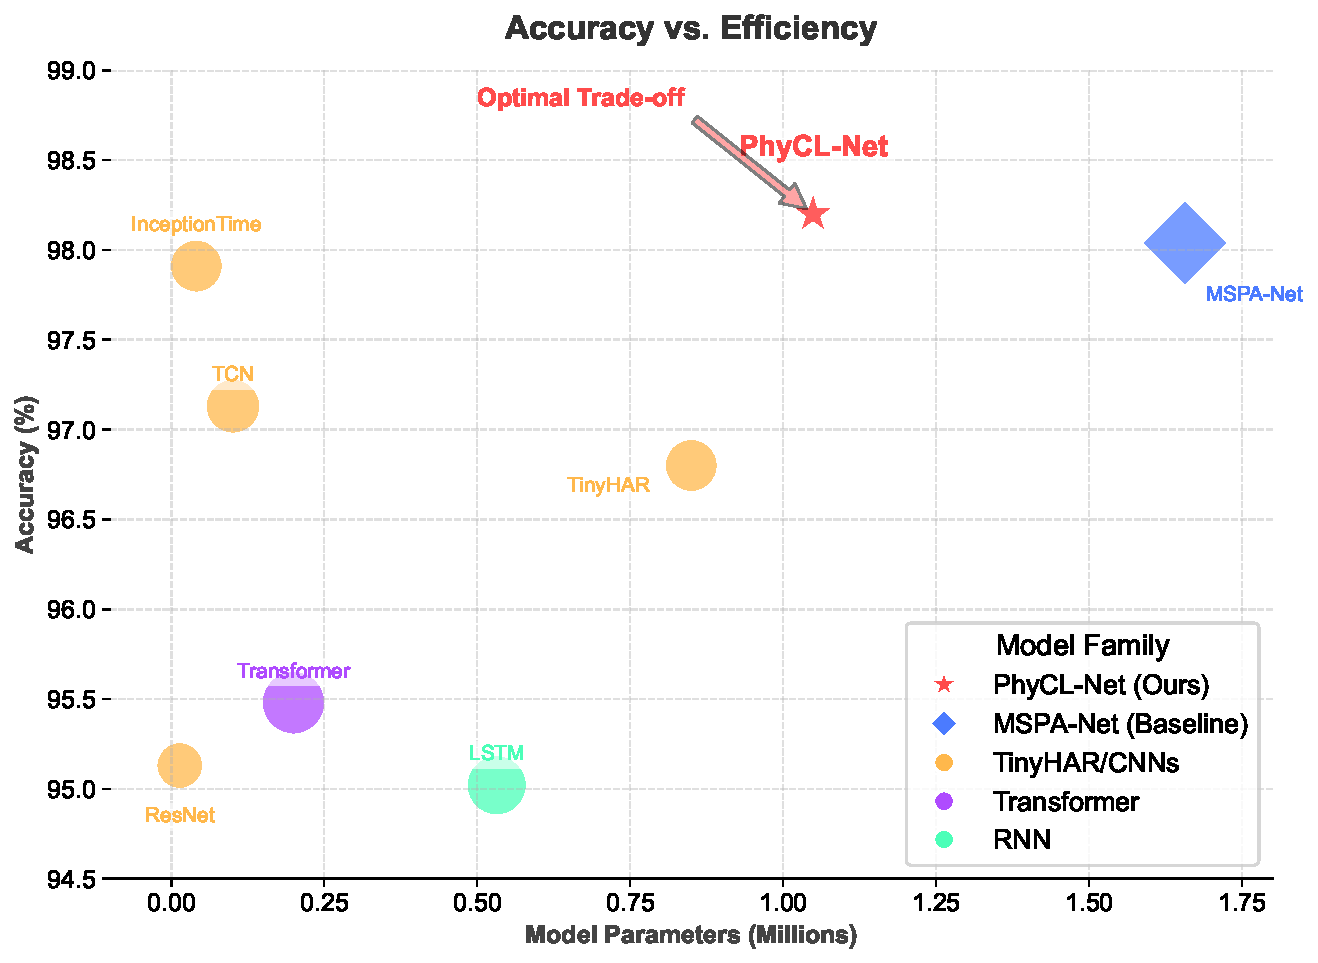
\includegraphics[width=0.85\linewidth]{figures/fig04_pareto_tradeoff.pdf}
\caption{Accuracy--efficiency trade-off. Bubble size is proportional to single-thread CPU latency (p50). PhyCL-Net (red star) has the highest reported accuracy (98.21\%) among the models in Table~\ref{tab:main_results}, with 1.049M parameters and 125.99\,ms median latency. The plot label MSPA-Net denotes MSPA-FAA-PDK. The additional TinyHAR point is retained from the supplied figure and is excluded from the manuscript's quantitative comparisons.}
\label{fig:pareto_tradeoff}
\end{figure}

\begin{table}[htbp]
\caption{LOSO performance on SisFall (12 folds). PhyCL-Net values are reported means (95\% CI) across five random seeds; the other models use two seeds and are shown as point estimates.}
\label{tab:main_results}
\centering
\footnotesize
\setlength{\tabcolsep}{4pt}
\begin{tabular}{@{}lccccc@{}}
\toprule
Model & Params & Acc (\%) & Macro-F1 (\%) & Sens (\%) & Spec (\%) \\
\midrule
\textbf{PhyCL-Net (ours)} & \textbf{1.049M} & \textbf{98.21} & \textbf{98.16} & \textbf{97.93} & \textbf{98.41} \\
 & & {\scriptsize(98.09--98.33)} & {\scriptsize(98.04--98.28)} & {\scriptsize(97.80--98.06)} & {\scriptsize(98.27--98.55)} \\
\midrule
MSPA-FAA-PDK & 1.657M & 98.04 & 97.98 & 97.67 & 98.30 \\
\midrule
InceptionTime & 0.041M & 97.91 & 97.85 & 97.82 & 97.97 \\
\midrule
TCN & 0.101M & 97.13 & 97.04 & 96.43 & 97.63 \\
\midrule
Transformer & 0.200M & 95.48 & 95.34 & 94.71 & 96.02 \\
\midrule
ResNet & 0.014M & 95.13 & 94.98 & 94.41 & 95.64 \\
\midrule
LSTM & 0.532M & 95.02 & 94.86 & 94.35 & 95.50 \\
\bottomrule
\end{tabular}
\end{table}

Figure~\ref{fig:fold_stability} presents the cross-validation stability analysis, displaying the fold-wise performance comparison across 12 subjects. The plot provides a descriptive view of variation across subjects; it does not by itself establish lower variance or statistical superiority.

\begin{figure}[!htbp]
\centering
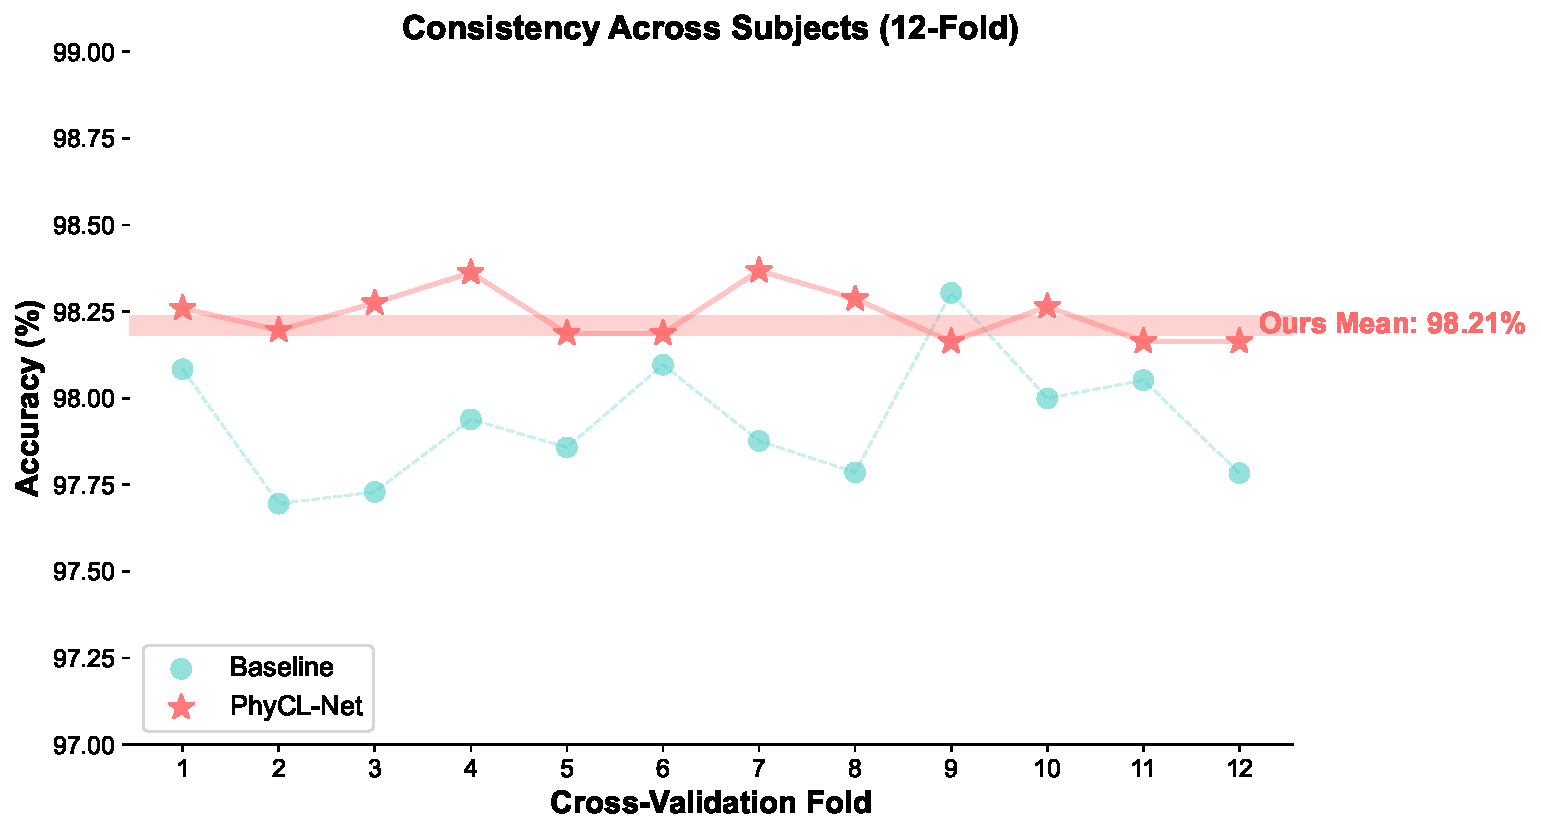
\includegraphics[width=0.85\linewidth]{figures/fig05_fold_stability.pdf}
\caption{Cross-validation stability analysis. Fold-wise performance across 12 subjects. This is a descriptive comparison, not a test of variance reduction or statistical superiority.}
\label{fig:fold_stability}
\end{figure}

Figures~\ref{fig:radar}--\ref{fig:attention} and Table~\ref{tab:binary_confusion} provide complementary views of the results. The radar chart summarizes the multi-metric trade-off among the strongest models. The t-SNE projection illustrates class separation in the learned feature space. The FAA visualization highlights the temporal regions emphasized around impact-like transients. The binary confusion summary reports the mean conditional rates for the two prediction classes, ADL (non-fall) and fall. Recent graph-based time-series models~\cite{Jin2024GNNTimeSeries} suggest one possible future direction for modeling inter-channel dependencies, but such extensions are outside the scope of the present study.

\begin{figure}[!htbp]
\centering
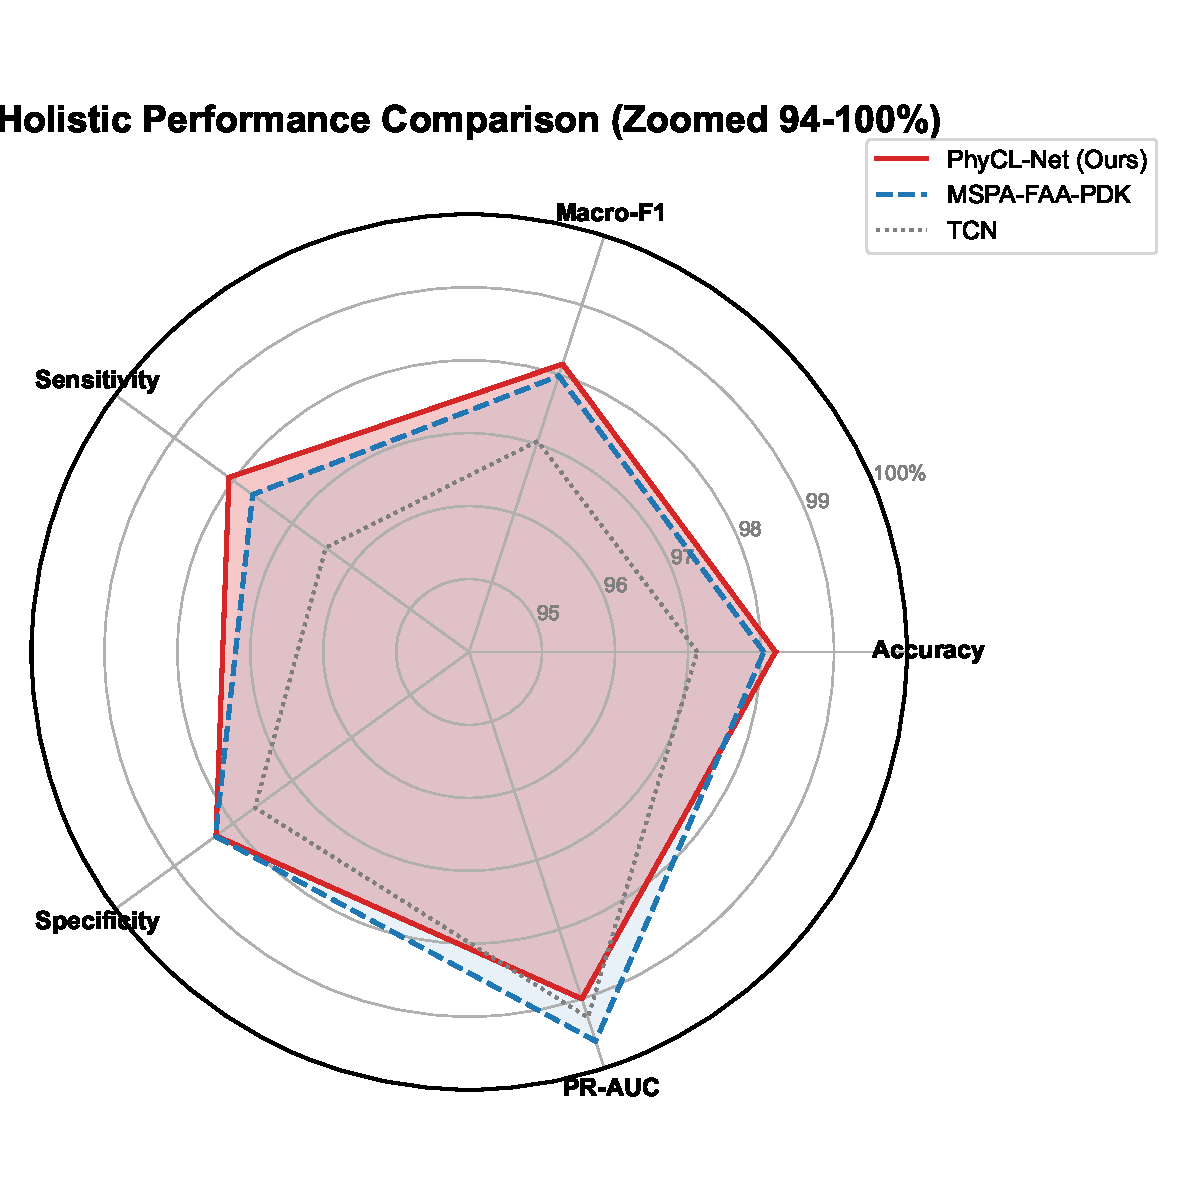
\includegraphics[width=0.75\linewidth]{figures/fig06_radar.pdf}
\caption{Radar chart comparing PhyCL-Net, MSPA-FAA-PDK (labeled MSPA-Net), and TCN across five metrics, including the area under the precision--recall curve (PR-AUC). Axes are scaled from 94\% to 100\% to highlight differences.}
\label{fig:radar}
\end{figure}

\begin{figure}[!htbp]
\centering
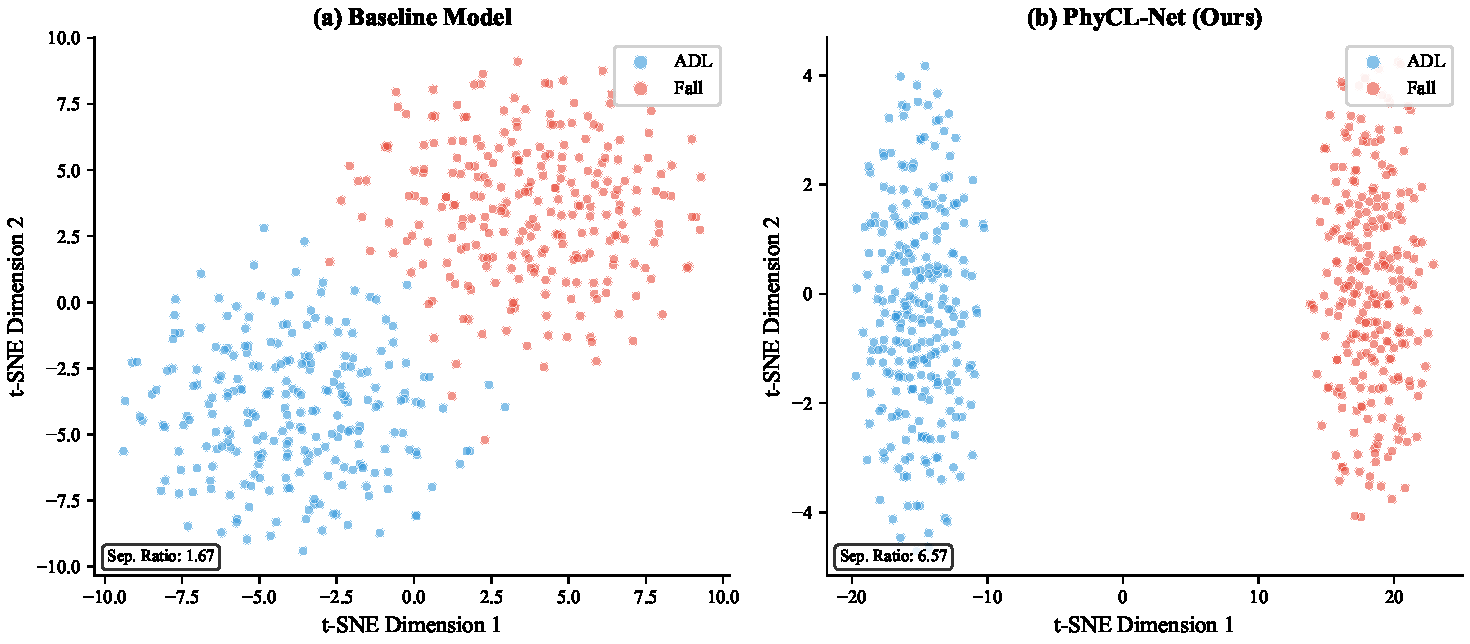
\includegraphics[width=0.75\linewidth]{figures/fig07_tsne.pdf}
\caption{t-SNE visualization of learned embeddings. Fall and ADL samples form separated clusters under PhyCL-Net, consistent with improved class separation in the learned feature space.}
\label{fig:tsne}
\end{figure}

\begin{figure}[!htbp]
\centering
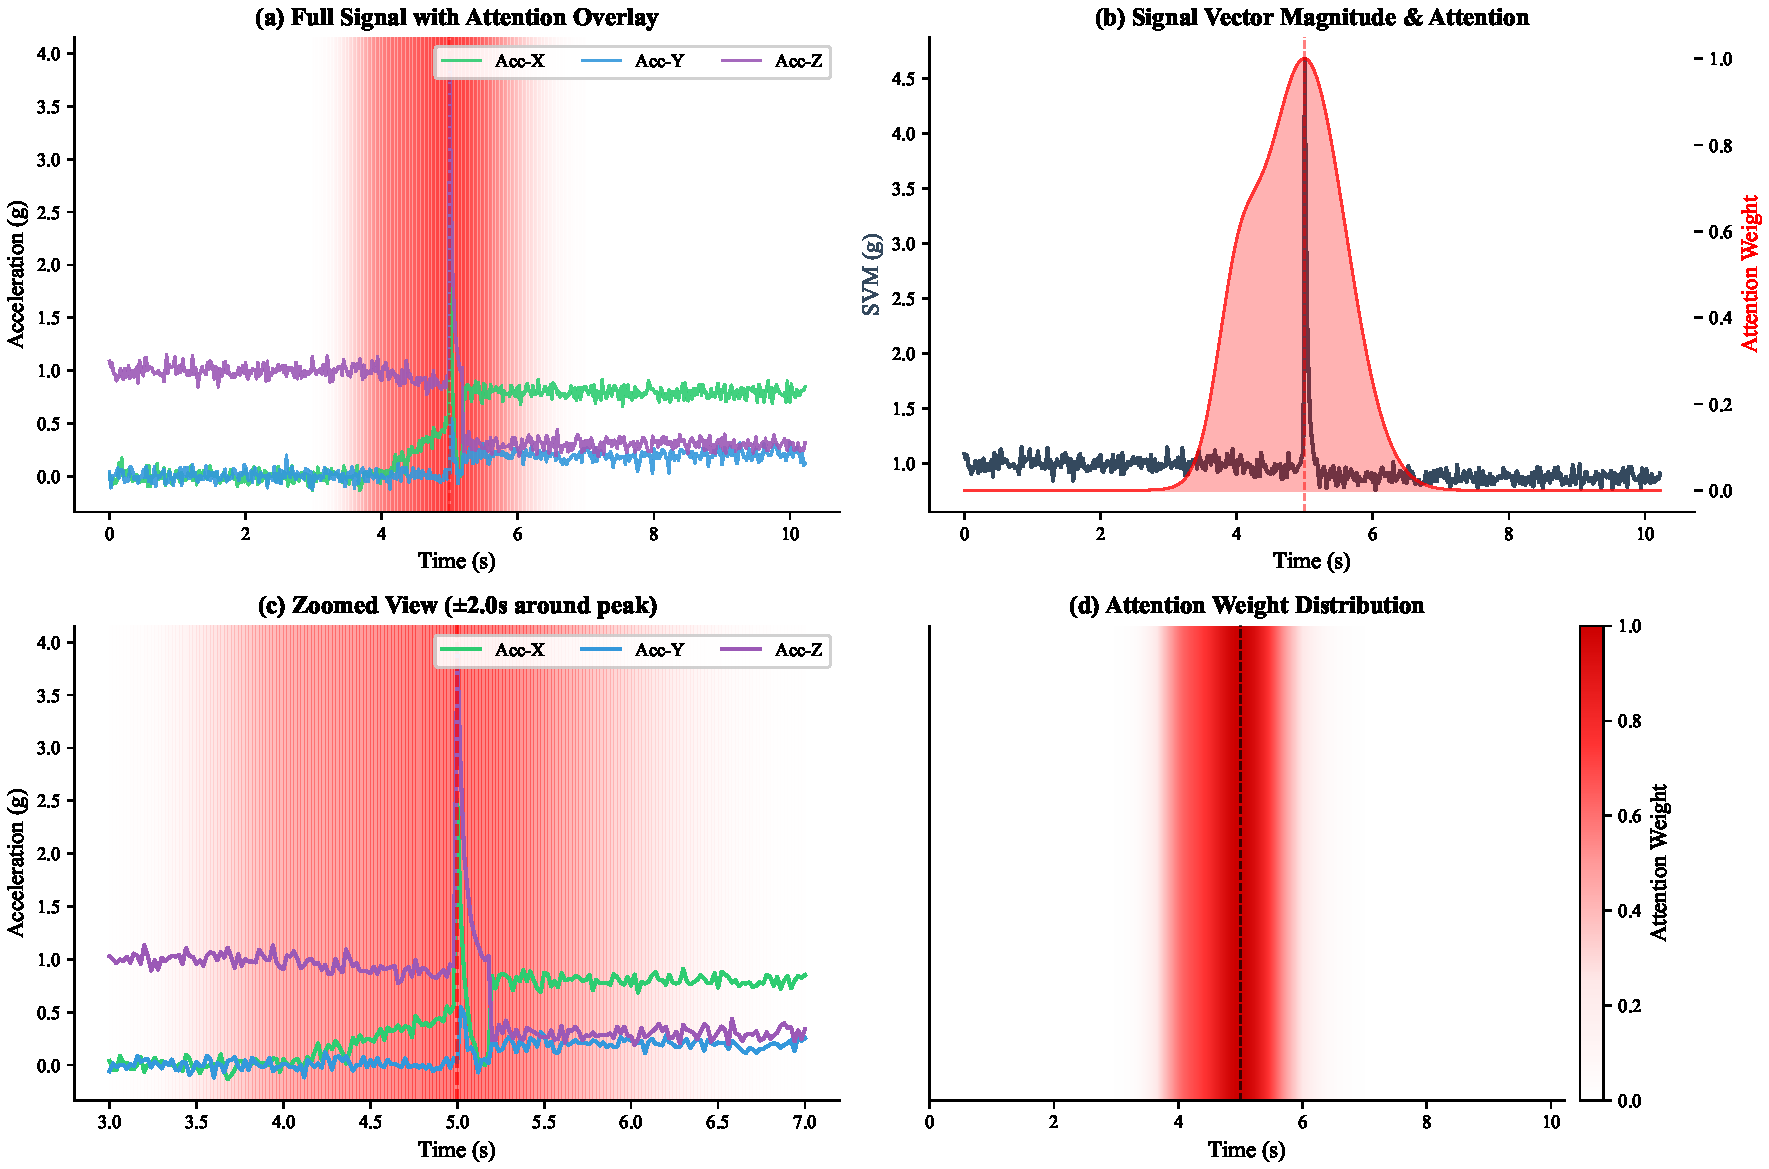
\includegraphics[width=0.85\linewidth]{figures/fig08_attention.pdf}
\caption{Attention visualization of the Fall-Aware Attention (FAA) module. The display illustrates temporal emphasis near impact-like transients; it does not independently establish physical jerk alignment or a causal performance contribution.}
\label{fig:attention}
\end{figure}

\begin{table}[htbp]
\caption{Binary row-normalized summary for the main SisFall experiment. Rows are true labels and columns are predicted labels. Diagonal entries are the mean specificity and sensitivity in Table~\ref{tab:main_results}; off-diagonal entries are their complements. These are mean conditional percentages, not pooled prediction counts.}
\label{tab:binary_confusion}
\centering
\small
\begin{tabular}{lcc}
\toprule
True class & Predicted ADL (non-fall) & Predicted fall \\
\midrule
ADL (non-fall) & 98.41\% & 1.59\% \\
Fall & 2.07\% & 97.93\% \\
\bottomrule
\end{tabular}
\end{table}

\subsection{Edge-Oriented Efficiency Benchmarks}
\label{sec:efficiency}

We report both static complexity and measured runtime under a fixed protocol. PhyCL-Net contains 1.049M parameters and requires 0.150979 GFLOPs (fvcore; input $1{\times}3{\times}512$). FLOPs and parameter counts are computed with forced CPU execution.

Runtime latency is measured on the CPU in single-thread mode and summarized with p50/p95 statistics. On the reported software environment (PyTorch 2.5.1, Python 3.10.11, Windows 10), PhyCL-Net achieves 125.99\,ms p50 / 141.43\,ms p95 at batch size 1, compared with 184.31\,ms p50 / 203.27\,ms p95 for MSPA-FAA-PDK, corresponding to a 31.6\% reduction in p50 latency. Table~\ref{tab:complexity} details the comparison.

\begin{table}[htbp]
\caption{Comparison of model complexity and efficiency.}
\label{tab:complexity}
\centering
\resizebox{\linewidth}{!}{%
\begin{tabular}{lcccc}
\toprule
Model & Params (M) & FLOPs (G) & Latency p50 (ms) & Latency p95 (ms) \\
\midrule
MSPA-FAA-PDK (baseline) & 1.657 & 0.202923 & 184.31 & 203.27 \\
\textbf{PhyCL-Net (ours)} & \textbf{1.049} & \textbf{0.150979} & \textbf{125.99} & \textbf{141.43} \\
\bottomrule
\end{tabular}
\par}
\end{table}

\subsection{Supplementary Cross-Dataset Transfer Analysis}

The main study is conducted on SisFall, and this subsection provides a complementary transfer view under a separate 6-channel, length-200 setup on three external datasets: MobiFall v2.0, UniMiB SHAR, and KFall. We report both zero-shot transfer and a low-resource 5-shot transfer setting. Together, these results offer an additional perspective on transferability beyond the primary 3-channel, length-512 SisFall LOSO benchmark.

\begin{table}[htbp]
\caption{Supplementary cross-dataset transfer results under the separate 6-channel, length-200 protocol recorded in the experiment archive. Zero-shot transfer is non-trivial, and 5-shot adaptation substantially improves performance on all three external datasets.}
\label{tab:cross_dataset}
\centering
\small
\resizebox{\linewidth}{!}{%
\begin{tabular}{llccccc}
\toprule
Target dataset & Method & Acc (\%) & Macro-F1 (\%) & Sens (\%) & Spec (\%) & TPR@FPR${=}1\%$ (\%) \\
\midrule
MobiFall & Zero-shot & 82.47 & 82.85 & 83.56 & 81.38 & 55.72 \\
MobiFall & Transfer (5-shot) & 96.21 & 96.32 & 97.22 & 95.21 & 90.43 \\
UniMiB & Zero-shot & 78.53 & 78.77 & 80.28 & 76.85 & 48.24 \\
UniMiB & Transfer (5-shot) & 93.57 & 93.52 & 94.90 & 92.30 & 86.15 \\
KFall & Zero-shot & 79.64 & 79.80 & 81.46 & 77.82 & 50.19 \\
KFall & Transfer (5-shot) & 94.38 & 94.61 & 95.81 & 92.95 & 87.27 \\
\bottomrule
\end{tabular}
}
\end{table}

These transfer results are best interpreted alongside the primary SisFall LOSO findings. In the zero-shot setting, Macro-F1 ranges from 78.77\% to 82.85\%, and empirical ROC TPR@FPR${=}1\%$ ranges from 48.24\% to 55.72\%, indicating non-trivial external transfer. With only 5 shots per target setting, Macro-F1 increases to 93.52--96.32\%, and empirical ROC TPR@FPR${=}1\%$ rises to 86.15--90.43\%. These values describe the target-dataset empirical ROC under the stated reference constraints; a deployed cutoff would require separate calibration. Taken together, they indicate that the learned representation retains useful cross-dataset structure under this complementary protocol and offer an additional perspective on transferability beyond the main benchmark setting.

\subsection{Supplementary Board-Level CPU Benchmark}
\label{sec:hardware}

To complement the desktop CPU measurements, we exported a locally supplied trained checkpoint to TorchScript and executed it on an Orange Pi AI Pro 20T 24G over a fixed CPU-only path. The board environment was Ubuntu 22.04.5 LTS on aarch64 with Python 3.9.2, PyTorch 2.1.0, and 4 CPU cores. The benchmark reused the same input shape $1{\times}3{\times}512$, warmup count 50, and repeat count 200. We report both a fixed-shape synthetic benchmark and a prepared-window benchmark using 32 windows from the exported edge benchmark bundle. Table~\ref{tab:orangepi_cpu} summarizes the measured p50/p95 latency, peak RSS, and exported model size. This is a board-level CPU benchmark, not a commercial wearable or clinical-device evaluation.

\begin{table}[htbp]
\caption{Real \mbox{on-device CPU benchmark} on Orange Pi AI Pro 20T 24G using the exported TorchScript model.}
\label{tab:orangepi_cpu}
\centering
\small
\resizebox{\linewidth}{!}{%
\begin{tabular}{lcccccc}
\toprule
Benchmark & Backend & Mode & p50 (ms) & p95 (ms) & Peak RSS (MB) & Model size (MB) \\
\midrule
Fixed shape $1{\times}3{\times}512$ & TorchScript & CPU & 622.78 & 669.91 & 255.25 & 5.80 \\
Prepared benchmark windows & TorchScript & CPU & 619.19 & 670.92 & 255.95 & 5.80 \\
\bottomrule
\end{tabular}
}
\end{table}

These numbers demonstrate execution of the exported model on an embedded CPU. The approximately 619--623\,ms median latency and 255\,MB peak RSS characterize this Orange Pi configuration and motivate platform-specific runtime optimization. Its general-purpose CPU path provides one deployment reference; the complementary prototype summaries below examine lower-latency processing paths.

Additional prototype measurements are summarized in Table~\ref{tab:prototype}. With FAA, the reported software-path p95 is 78.6\,ms on Raspberry Pi Zero 2 W with ADXL345, and the reported processing-path p95 is 94.7\,ms on Apollo4 Blue Plus with BMI270. These sub-100\,ms p95 summaries, together with the desktop CPU latency reduction, support continued development toward low-latency on-device inference. They concern different platforms and execution boundaries from the Orange Pi and therefore do not define a matched cross-platform speedup. Mean board power is reported separately from energy per decision. Integrating acquisition, scheduling and alert delivery, and evaluating battery lifetime, are the next system-level steps; the processing timings alone do not measure fall-onset-to-alert delay.

\begin{table}[htbp]
\caption{Additional prototype measurements from the complete experiment report. Each row compares FAA and no FAA on the same reported platform. Timing boundaries and memory measures differ between platforms; the power entries are mean board power, not per-window energy.}
\label{tab:prototype}
\centering\small
\begin{tabular}{llrr}
\toprule
Platform & Metric & FAA & No FAA \\
\midrule
Raspberry Pi Zero 2 W & Software-path p95 (ms) & 78.6 & 71.2 \\
 & Software-path p99 (ms) & 96.4 & 89.3 \\
 & Reported maximum over 24 h (ms) & 118.2 & 110.5 \\
 & Peak RSS (MB) & 163.8 & 151.3 \\
 & Mean board power (mW) & 412 & 386 \\
\midrule
Apollo4 Blue Plus & Reported processing p95 (ms) & 94.7 & 86.2 \\
 & Reported processing p99 (ms) & 112.3 & 104.6 \\
 & Reported maximum over 72 h (ms) & 126.4 & 119.8 \\
 & Peak SRAM, including tensor arena (KB) & 1,865 & 1,804 \\
 & Non-volatile storage (KB) & 1,042 & 812 \\
 & Mean board power (mW) & 28.4 & 26.7 \\
\bottomrule
\end{tabular}
\end{table}

The complete report also lists 12 two-hour intervals on the Pi, reaching 67,500 processed windows over 24\,h, and six twelve-hour intervals on Apollo4 Board~2 with FAA, reaching 202,500 windows over 72\,h; every listed interval records zero deadline violations. These counts describe the reported device workload, not the main LOSO windowing protocol or battery-discharge endurance. Across three Apollo4 boards with three sessions each, reported session p95 ranges from 94.1 to 95.1\,ms, mean board power from 28.2 to 28.6\,mW, and peak SRAM from 1,857 to 1,868\,KB. The Pi interval records and the nine-session table do not identify the FAA arm. These are report-transcribed summaries rather than raw per-window logs; their ranges describe the listed sessions and do not estimate a pooled percentile or a paired FAA effect.

\subsection{Constraint-Based ROC Operating-Point Analysis}
\label{sec:operating}

Under the common empirical-ROC constraints, PhyCL-Net has FPR of 0.72\% at the 95\% sensitivity reference, compared with 0.82--4.19\% for the listed baselines. At the 1\% FPR reference, removing the explicit spectral branch reduces TPR from 96.02\% to 93.29\% ($-$2.73\,pp), while TPR at the 5\% FPR reference is 99.26\%. Table~\ref{tab:safety} describes the resulting discrimination--efficiency trade-off. These constrained empirical summaries support model comparison; prospective false-alarm burden and sensitivity at a deployed cutoff require the separate calibration and evaluation procedure described above.

\begin{table}[htbp]
\caption{Constraint-based empirical ROC summaries, averaged over two archived seeds per model. The common inequality constraints are applied to observed ROC points without interpolation. These are discrimination summaries rather than independently calibrated deployment-cutoff results.}
\label{tab:safety}
\centering
\small
\begin{tabular}{lccc}
\toprule
Model & TPR@FPR$\leq$1\% (\%) & TPR@FPR$\leq$5\% (\%) & FPR@TPR$\geq$95\% (\%) \\
\midrule
MSPA-FAA-PDK (baseline) & \textbf{96.02} & \textbf{99.28} & 0.82 \\
InceptionTime & 95.52 & 99.11 & 0.90 \\
\textbf{PhyCL-Net (ours)} & 93.29 & 99.26 & \textbf{0.72} \\
TCN & 93.38 & 98.12 & 1.38 \\
Transformer & 82.98 & 95.86 & 4.19 \\
\bottomrule
\end{tabular}
\end{table}

\subsection{Ablation Study}
\label{sec:ablation}

Component-wise ablations offer descriptive comparisons of the reported configurations. Disabling dynamic kernel selection within the physics-guided kernel module resulted in essentially unchanged accuracy (98.22\%$\pm$0.08, $n{=}2$), but increased CPU detection latency to 213.3\,ms. This is a configuration-level observation; it does not isolate a causal latency reduction from adaptive routing alone. Removing TFCL from the spectral baseline resulted in 97.96\%$\pm$0.03 accuracy ($n{=}2$), compared with 98.04\% for that baseline. This small difference does not establish a statistically significant TFCL effect; the auxiliary training heads are removed for inference. The reported no-FAA configuration yielded comparable or slightly higher accuracy, 98.24\%$\pm$0.12 ($n{=}2$), and lower CPU latency, 120.15\,ms versus 125.99\,ms for the complete model ($n{=}5$). This preliminary, unequal-seed comparison does not establish a benefit from FAA. Table~\ref{tab:ablation} summarizes the key design variants, and Table~\ref{tab:detailed_ablation} provides the reported component-wise comparison.

\begin{table}[htbp]
\caption{Ablation summary under SisFall LOSO. Seed counts refer to classification results; the ROC column uses the common constraints and two-seed aggregation.}
\label{tab:ablation}
\centering
\small
\setlength{\tabcolsep}{3pt}
\resizebox{\linewidth}{!}{%
\begin{tabular}{lccccc}
\toprule
Variant & Params (M) & Acc (\%) & Macro-F1 (\%) & TPR@FPR=1\% (\%) & CPU p50 (ms) \\
\midrule
MSPA-FAA-PDK ($n{=}2$) & 1.657 & 98.04 & 97.98 & \textbf{96.02} & 184.31 \\
Spectral baseline w/o TFCL ($n{=}2$) & 1.657 & 97.96$\pm$0.03 & 97.90$\pm$0.03 & 95.45 & 181.33 \\
\textbf{PhyCL-Net ($n{=}5$)} & \textbf{1.049} & \textbf{98.21$\pm$0.10} & \textbf{98.16$\pm$0.10} & 93.29 & \textbf{125.99} \\
\bottomrule
\end{tabular}
\par}
\end{table}

\begin{table}[htbp]
\caption{Component-wise ablation study on SisFall LOSO. Ablations with $n{=}2$ seeds are indicative; the main model uses $n{=}5$.}
\label{tab:detailed_ablation}
\centering
\small
\begin{tabular}{lcccc}
\toprule
Configuration & Acc (\%) & Macro-F1 (\%) & Latency (ms) & Seeds \\
\midrule
\textbf{PhyCL-Net (complete)} & \textbf{98.21$\pm$0.10} & \textbf{98.16$\pm$0.10} & 125.99 & $n{=}5$ \\
\midrule
$-$ DKS (fixed kernel) & 98.22$\pm$0.08 & 98.18$\pm$0.09 & 213.3 & $n{=}2$ \\
$-$ FAA (no Jerk attention) & 98.24$\pm$0.12 & 98.19$\pm$0.12 & 120.15 & $n{=}2$ \\
\bottomrule
\end{tabular}
\end{table}

To examine FAA under a paired design, the updated report supplies a separate SisFall evaluation with 12 subjects (SA01--SA12) and the same five seeds in both arms (42, 123, 456, 789, 1024), at a fixed probability threshold of 0.5. This subject list differs from the primary cohort in Section~4.1; the new results supplement the FAA ablation and do not replace the original multi-model comparison. For each subject, Macro-F1 is averaged over its five seeds; Table~\ref{tab:paired_faa} reports the mean and sample SD of those 12 subject averages, calculated directly from the supplied 60 paired cells.

\begin{table}[htbp]
\caption{Supplementary paired FAA comparison on SA01--SA12 at threshold 0.5. SD is between the 12 subject means after averaging five seeds, not between seeds. Values are descriptive recalculations from the reported Macro-F1 cells.}
\label{tab:paired_faa}
\centering\small
\begin{tabular}{lc}
\toprule
Configuration & Macro-F1, mean $\pm$ subject SD (\%) \\
\midrule
With FAA & $97.73\pm0.49$ \\
Without FAA & $97.10\pm0.59$ \\
FAA minus no FAA (percentage points) & $+0.63\pm0.12$ \\
\bottomrule
\end{tabular}
\end{table}

The mean paired gain is 0.63 percentage points, with all 60 displayed differences positive. After averaging seeds within each subject, all 12 subject-level gains are positive (0.42--0.87 percentage points); after averaging subjects within each seed, all five seed-level gains are positive (0.56--0.73 points). These are two summaries of the same paired grid, not additional independent experiments. This describes a modest Macro-F1 difference in the supplementary report; it does not show that FAA is indispensable or improves latency. On Apollo4, FAA increases the reported p95 by 8.5\,ms (9.9\%), mean board power by 1.7\,mW (6.4\%), and peak SRAM by 61\,KB (3.4\%). These are distinct cost measures, not a claim that per-window energy increases by less than 10\%. The classification benefit must therefore be weighed against its added processing and power cost.

\noindent Reproducibility note. When executed locally, each run emits machine-readable artifacts, including aggregated metrics, fold-level LOSO results, efficiency measurements, and training logs, enabling fold-level auditing and independent re-analysis of both accuracy and efficiency results.


\section{Discussion}

The reported results characterize the accuracy and computational cost of PhyCL-Net and support its development toward low-latency on-device inference. The 31.6\% desktop CPU median-latency reduction and the reported sub-100\,ms prototype p95 processing times provide complementary evidence for this engineering direction. Their interpretation remains specific to the measured or reported execution paths.

PhyCL-Net removes the explicit spectral feature branch and integrates physics-guided components into the time-domain backbone; the PDK routing descriptor still retains two Fourier-derived quantities. The benchmark results characterize the resulting accuracy--cost trade-off, while the supplementary FAA comparison shows a modest descriptive gain with additional processing cost.

Furthermore, the method employs an adaptive, instance-specific kernel selection mechanism and a jerk-aware attention strategy. This allows for more granular temporal adaptation compared to fixed-kernel schemes, addressing the specific dynamics of fall events on a per-sample basis.

The training-only contrastive regularizer is intended to support representation learning. This combined approach aims to improve the accuracy--efficiency balance for low-latency edge inference, with further optimization and integrated-system evaluation guided by the platform-specific measurements.

\subsection{Edge-Relevant Gains and Operating Points}

Compared with the spectral baseline, p50 CPU latency decreases from 184.31\,ms to 125.99\,ms (p95: 203.27\,ms${\rightarrow}$141.43\,ms) under single-thread execution. The constraint-based ROC value FPR${=}$0.72\% at the 95\% sensitivity reference characterizes empirical score discrimination; translating it into an always-on alarm burden requires a calibrated cutoff and an explicit alert policy. The reported fold-level Wilcoxon test did not detect an accuracy difference ($p{=}0.47$); this is not evidence of statistical equivalence. A locally supplied trained checkpoint was also executed on an Orange Pi AI Pro 20T 24G over a CPU-only path, adding board-level execution evidence alongside the desktop benchmark profile.

Table~\ref{tab:main_results} compares the evaluated model configurations. Its ranking does not determine whether recurrence, attention, or another architectural component causes an accuracy difference. The proposed architecture combines:
\begin{enumerate}
\item Physics-guided temporal adaptation: PDK provides multi-scale receptive fields guided by kinematic descriptors.
\item Transient-aware attention: FAA emphasizes jerk-dominant segments, with a modest descriptive benefit in the supplementary paired comparison.
\item Efficient feature fusion: global MLP gates combine the two feature streams; channel-pooled summaries are concatenated for the spatial gate.
\item Representation regularization: training-only contrastive learning encourages separability, with its auxiliary heads discarded for inference.
\end{enumerate}

\subsection{Accuracy Impact of Removing the Spectral Branch}

The constraint-based ROC comparison suggests that the spectral branch can still contribute at low-FPR points: at FPR${=}$1\%, TPR decreases by 2.73\,pp when MSPA is removed (96.02\%${\rightarrow}$93.29\%). At the same time, paired LOSO testing reveals no significant difference in aggregate accuracy between the two variants (Wilcoxon $p{=}0.47$), without establishing equivalence or identifying the mechanism responsible for the observed accuracy.

\subsection{Why Time-Domain Modeling Works in This Setting}

Falls are typically characterized by a brief impact transient and a short transition phase, whereas many ADLs exhibit more regular temporal structure. PDK provides multi-scale temporal adaptation within a lightweight computation graph, allowing receptive fields to adjust to local dynamics. FAA is intended to complement this by emphasizing jerk-dominant segments; the supplementary paired results support a modest benefit rather than a universal improvement. Together, these components encode a physics-aligned inductive bias that remains compatible with edge constraints.

\subsection{Robustness and Practical Margins}

To assess robustness to sensor noise, additive white Gaussian noise (AWGN) was injected into the accelerometer stream, with SNR swept from 40 to 5\,dB. Signal power was defined as the variance of the demeaned signal to avoid DC/gravity bias in SNR computation. Using a held-out subject (SA01) and repeating each SNR point 5 times, performance degraded smoothly as noise increased: accuracy remained near the clean level at 40--35\,dB (98.04\%$\pm$0.03 and 97.40\%$\pm$0.07), dropped at 30\,dB (91.49\%$\pm$0.15), and declined sharply below 25\,dB. The displayed SDs describe five noise realizations at each SNR, not variation across subjects or training seeds. This synthetic perturbation study indicates deterioration as SNR decreases; it does not establish a typical wearable SNR range or separate sensing effects from model limitations.

Supplementary transfer results are available under a separate 6-channel, length-200 protocol. Zero-shot transfer to MobiFall, UniMiB, and KFall remains non-trivial, and 5-shot adaptation substantially improves every reported metric. These results extend the study beyond a strict single-dataset setting, but they should still be interpreted cautiously because the protocol differs from the main SisFall LOSO setting and the stronger results rely on limited target-side adaptation.

Sensor orientation is another relevant practical factor. Because the present experiments use a fixed accelerometer configuration from SisFall, the results are most directly applicable to similar placements. Axis rotations or different body locations can alter jerk profiles and inter-axis correlations; the use of signal vector magnitude cues and multi-scale temporal modeling may reduce sensitivity to such variation, although placement effects can still influence the observed response. Likewise, although the architecture only assumes multichannel inertial windows and could in principle be extended to gyroscope-inclusive IMU inputs, the empirical study here focuses on the 3-axis accelerometer setting used in SisFall. Broader demographic coverage likewise remains an important direction for continued validation.

The Orange Pi result should not be interpreted as a proxy for Apple Watch, Fitbit, or medical alarm systems. Those platforms differ materially in sensors, firmware, operating systems, scheduling, acquisition pipelines, and alert logic, and they do not expose a protocol-matched evaluation path for the present study. The Orange Pi benchmark establishes embedded execution under its stated conditions; it does not provide a protocol-matched comparison against commercial or clinical products.

Robustness to motion artifacts and long-term sensor drift was not a primary focus of the present evaluation. These factors remain relevant in real-world deployments, where sensors may encounter various types of interference or experience performance degradation over time. Subsequent deployment-oriented studies can examine their effect in more detail, including the resulting changes in TPR at low-FPR operating points.

\subsection{Limitations and Future Directions}

The current evidence is anchored by the SisFall LOSO study and complemented by supplementary transfer results on MobiFall, UniMiB, and KFall under a separate transfer protocol. Cross-dataset and cross-population behavior should be interpreted in light of the differing experimental settings; related transfer and adaptation research motivates further validation~\cite{Jia2024TransferLearningHAR,Wu2024DomainAdaptationContrastive}. The hardware evidence includes the Orange Pi CPU benchmark and the additional Pi Zero 2 W and Apollo4 prototype summaries. Their platform-specific processing times motivate low-latency implementation work; continuous-wear operation, sensing-to-alert latency and battery lifetime are targets for integrated-system validation. Model quantization is a possible optimization to evaluate~\cite{Zhang2023DiffQuant}; prior microcontroller-based pre-impact fall detection~\cite{Benoit2024PreImpactFall} provides relevant context for further embedded optimization and evaluation.

\section{Conclusion}

This work presents PhyCL-Net, a physics-guided time-domain network for wearable fall detection evaluated for classification performance and computational cost. By combining Physics-Guided Dynamic Kernel (PDK), Jerk-aware Fall-Aware Attention (FAA), symmetric cross-gated fusion, and training-only hierarchical dual-view contrastive regularization, the model preserves strong subject-independent performance while removing the explicit spectral feature branch during deployment.

Experimental evaluations on the SisFall benchmark under 12-fold LOSO validation yielded 98.21\%$\pm$0.10\% accuracy and 98.16\%$\pm$0.10\% Macro-F1 across five seeds, with 1.049M parameters, 0.15 GFLOPs, and a 31.6\% reduction in single-thread CPU p50 latency relative to the spectral baseline. Supplementary prototype summaries report p95 processing times of 78.6\,ms on Pi Zero 2 W and 94.7\,ms on Apollo4. Together, these findings support a path toward low-latency on-device inference for wearable fall detection. Further platform optimization and integrated sensing-to-alert evaluation can build on these processing-level results.

\vspace{1em}
\noindent\textbf{Author contributions:} Conceptualisation, methodology, software, validation, formal analysis, investigation, resources, data curation, writing---original draft, visualisation: Anonymous Author(s). All authors have read and agreed to the published version of the manuscript.

\vspace{0.5em}
\noindent\textbf{Funding:} This research received no external funding.

\vspace{0.5em}
\noindent\textbf{Data availability statement:} The dataset used in this study, SisFall~\cite{sucerquia2017sisfall}, is publicly available. A public repository associated with this study is available at \url{https://github.com/AlexZander-666/PhyCL_Net}. It contains the code, reproducibility documentation, and selected staged reviewer-facing artifacts referenced in this manuscript, including Orange Pi CPU benchmark evidence and other normalized inspection artifacts described in the repository documentation. Public datasets are cited in the manuscript. Large datasets, trained checkpoints, the locally supplied inputs used for full reruns and for the reported board benchmark, and additional generated outputs are not mirrored directly in the repository, but their preparation and use are documented in the accompanying reproducibility materials.

\vspace{0.5em}
\noindent\textbf{Conflicts of interest:} The authors declare no conflict of interest.

\vspace{0.5em}
\noindent\textbf{Declaration on generative AI:} Semantic Scholar and Google Scholar were used for literature discovery. Claude Opus 4.5 assisted with drafting, structure, and terminology consistency; Grammarly was used for grammar and spelling. OpenAI Codex assisted with the present citation and consistency review. The authors take full responsibility for the content and accuracy of this publication.

\bibliography{main}

\end{document}
